

\chapter{Data Structures}


\section{Time Complexity}

\section{Space Complexity}



\section{Containers}

Arrays and vectors are the most common containers, I think. Arrays are fixed-size stack-based containers. Vectors
are dynamic containers.

\subsection{Containers Functions}

\begin{verbatim}
begin()         - returns an iterator on the first element 
end()           - returns an iterator after the last element
cbegin()        - version constant of begin() and end()
cend()  
rbegin()        - returns a reverse iterator pointing to the last element of a container
rend()          - returns an iterator pointing to one position before the beginning
before_begin()  - Only for forward_list! 
                  returns an iterator pointing to the position
                  before the first element in a container.  
cbefore_begin() - Only for forward_list!
                  Constant version of before_begin()

#include <vector>

int main() {
    std::vector<int> numbers{1, 2, 3, 4, 5};

    // Using rbegin() to iterate over elements in reverse order
    for (auto it = numbers.rbegin(); it != numbers.rend(); ++it) {
        std::cout << *it << " ";
    }

        // 5 4 3 2 1

    return 0;
}

#include <forward_list>

int main() {
    std::forward_list<int> numbers{2, 3, 4};

    // Inserting an element at the beginning using before_begin()
    numbers.insert_after(numbers.before_begin(), 1);

    // Printing the elements
    for (auto it = numbers.begin(); it != numbers.end(); ++it) {
        std::cout << *it << " ";
    }
    
        // 1 2 3 4

    return 0;
}


Forward_list doesn't have support for rbegin() / rend() or
crbegin() / crend()
\end{verbatim}


\subsection{Container Iterations}

For Jason Turner, this construct, was one of the most difficult things to learn!

\begin{verbatim}
void print_map(const std::map<int, std::string> &map,
               const std::string &key_desc = "key",
               const std::string &value_desc = "value")
{
    for (std::map<int, std::string>::const_iterator data_itr = map.begin(); // this right here
         data_itr != map.end();
         ++data_itr)
    {
        std::cout << key_desc << ": '" << data_itr->first << "' "
                  << value_desc << ": '" << data_itr->second << "'\n";
    }
}

void print_map(const std::map<int, std::string> &map,
               const std::string &key_desc = "key",
               const std::string &value_desc = "value")
{
    for (auto data_itr = map.begin();
         data_itr != map.end();
         ++data_itr)
    {
        std::cout << key_desc << ": '" << data_itr->first << "' "
                  << value_desc << ": '" << data_itr->second << "'\n";
    }
}

// If only there was some simple way to iterate over all the values in a container.....
\end{verbatim}

\subsection{Containers Looping Mismatched}

\begin{verbatim}
for (auto itr = container.begin();
    itr != container2.end();
    ++itr) {
    // oops! most of us have done this at some point
}
\end{verbatim}

\subsection{Container Size functions}

\begin{verbatim}
size()     - returns the number of elements
             not available for forward_lists
max_size() - returns the maximum amount of elements that can be
             stocked in a container
resize()   - resize the container, to a new capacity
             not available for arrays
empty()    - returns true if container is empty, else false
\end{verbatim}

\subsection{Access and Research functions}

\begin{verbatim}

insert()
    numbers.insert(numbers.begin(), 0); 
    numbers.insert(numbers.begin() + 3, 10);
    numbers.insert(numbers.begin() + 2, {7, 8, 9});

push_back() / pop.back()
    std::vector<int> vec = {1, 2, 3, 4, 5};
    int newValue = 6;
    vec.push_back(newValue);


#include <list>
#include <algorithm>

struct Person {
    std::string name;
    int age;

    Person(const std::string& n, int a) : name(n), age(a) {}
};

int main() {
    std::list<Person> people;

    // Inserting elements in sorted order based on age
    people.insert(people.begin(), {"Alice", 25});
    people.insert(people.begin(), {"Bob", 30});
    people.insert(people.begin(), {"Charlie", 20});

    // Inserting an element after finding a specific person
    auto it = std::find_if(people.begin(), people.end(), [](const Person& p) {
        return p.name == "Bob";
    });
    if (it != people.end()) {
        people.insert(std::next(it), {"David", 27});
    }
\end{verbatim}

\subsection{static\_cast}

Used with enums to convert between different enum types or to convert an enum value to an integer type.
It allows for explicit and controlled type conversions, providing better type safety

\begin{verbatim}
int main() {
    Fruit selectedFruit = Fruit::Banana;
    int fruitIndex = static_cast<int>(selectedFruit);

    std::cout << "Selected fruit: " << fruitNames[fruitIndex] << std::endl;

    return 0;
}
\end{verbatim}


\section{Maps}

Dynamically resizing containers.

Unlike arrays, fixed sizes, std::map has an arbitrary number of key-value pairs.
`std::map` is a balanced binary search tree, it keeps elements sorted based on the keys, 
Insertions, deletions and searches have logarithmic time complexity.
Plus, keys must be unique within the map.

C++'s equivalent to Ruby's hash object. 
Both `std::map` and Ruby's hash are associative containers that store key-value pairs.
They allow efficient lookup and retrieval of values based on a given key.
The key-value pairs are stored in an unordered, unspecific manner.

\begin{verbatim}
#include <map>

int main() {
    std::string str = "hello";
    std::map<char, int> charFreq;

    // Count the frequency of each character in the string
    for (char c : str) {
        charFreq[c]++;
    }

    // Display the character frequencies
    for (const auto& pair : charFreq) {
        std::cout << pair.first << ": " << pair.second << std::endl;
    }

    return 0;
}

#include <map>
#include <string>

int main() {
    std::map<std::string, int> studentGrades;

    // Add student names and their grades
    studentGrades["Alice"] = 90;
    studentGrades["Bob"] = 85;
    studentGrades["Charlie"] = 95;

    // Access and display individual student grades
    std::cout << "Charlie's grade: " << studentGrades["Charlie"] << std::endl;

    // Iterate over all student grades
    for (const auto& pair : studentGrades) {
        std::cout << pair.first << ": " << pair.second << std::endl;
    }

    return 0;
}

std::map<int, Product> map1 {
    {1, Product(1, "Item 1")},
    {2, Product(10, "Item 2")},
};

map1[3] = Product(30, "Item 3");
for (std::pair<int, Product> elt : map1)
{
    cout << elt.first << " ";
    cout << elt.second.name << '\n';

}


#include <map>
#include <sstream>
#include <string>

int main() {
    std::string text = "lorem ipsum dolor sit amet, consectetur adipiscing elit.";

    // convert text to lowercase
    for (char& c : text) {
        c = std::tolower(c);
    }

    std::map<std::string, int> wordfreq;
    std::istringstream iss(text);
    std::string word;

    // count the frequency of each word in the text
    while (iss >> word) {
        wordfreq[word]++;
    }

    // display the word frequencies
    for (const auto& pair : wordfreq) {
        std::cout << pair.first << ": " << pair.second << std::endl;
    }

    return 0;
}

// Understand how this code is working
// Accidental copy?

std::map<std::string, int> get_map();

using element_type = std::pair<std::string, int>;

for (const element_type & : get_map())
{}
\end{verbatim}

 
\subsection{Maps Overview (Strengths, Weaknesses, Sorting and Uniqueness)}

\subsection{Maps Operations (Create Read Update Delete)}

\begin{verbatim}
    Create (Insert Key-Value Pair):
        map[key] = value 
        map.insert(std::make_pair(key, value))

    Read (Retrieve a value by key):
        Value = map[key]
        Checking if a key exists: map.count(key)

    Update (Modify the value of a key):
        map[key] = new_value

    Delete (Remove a key-value pair):
        map.erase(key)
        Removing all elements: map.clear()

#include <map>

int main() {
    std::map<int, std::string> map;

    // Create (Insert)
    map[1] = "Apple";
    map.insert(std::make_pair(2, "Banana"));

    // Read (Retrieve)
    std::cout << "Value at key 1: " << map[1];
    std::cout << "Key 2 exists? " << (map.count(2) ? "Yes" : "No");

    // Update
    map[1] = "Apricot";

    // Delete
    map.erase(2);

    // Display all key-value pairs
    for (const auto& pair : map) {
        std::cout << "Key: " << pair.first << ", Value: " << pair.second << std::endl;
    }

    return 0;
}
\end{verbatim}

\subsection{Multimaps}

A multimap allows multiple values to be associated with the same key. 

\begin{verbatim}
#include <map>

int main() {
    std::multimap<int, std::string> myMultimap;

    // Insert key-value pairs into the multimap
    myMultimap.insert(std::make_pair(1, "Apple"));
    myMultimap.insert(std::make_pair(2, "Banana"));
    myMultimap.insert(std::make_pair(1, "Apricot"));

    for (const auto& pair : myMultimap) {
        std::cout << "Key: " << pair.first << ", Value: " << pair.second << std::endl;
    }

        // Key: 1, Value: Apple
        // Key: 1, Value: Apricot
        // Key: 2, Value: Banana

    return 0;
}
\end{verbatim}

\section{Sets}

Std::set represents a sorted set of unique elements. The set maintains a sorted order,
the elements are automatically sorted. Plus, it makes sure they are unique.

\begin{verbatim}
#include <set>

int main() {
    std::set<int> mySet;
    mySet.insert(5);
    mySet.insert(2);
    mySet.insert(8);

    for (const auto& element : mySet) {
        std::cout << element << " ";
    }
    std::cout << std::endl;

    // Check if an element exists in the set
    int searchElement = 2;
    if (mySet.count(searchElement) > 0) {
        std::cout << searchElement << " exists in the set" << std::endl;
    } else {
        std::cout << searchElement << " does not exist in the set" << std::endl;
    }

    // Remove an element from the set
    int removeElement = 5;
    mySet.erase(removeElement);

    for (const auto& element : mySet) {
        std::cout << element << " ";
    }
    std::cout << std::endl;
    
    // 2 5 8
    // 2 exists in the set
    // 2 8

    return 0;
}
\end{verbatim}

\subsection{Multisets}

Std::multiset represents a sorted set of elements (duplicates are possible). The set maintains a sorted order,
the elements are automatically sorted.

\begin{verbatim}
#include <iostream>
#include <set>

int main() {
    std::multiset<int> myMul;
    myMul.insert(5);
    myMul.insert(2);
    myMul.insert(2); // Duplicates are allowed in a multiset

    for (const auto& element : myMul) {
        std::cout << element << " ";
    }
    std::cout << std::endl;

    // Check the count of a specific element
    int countE = 2;
    std::cout << countE << " appears " << myMul.count(countE) << " times" << '\n';

    // Remove specific elements
    int removeElement = 2;
    myMul.erase(removeElement);

    for (const auto& element : myMul) {
        std::cout << element << " ";
    }
    std::cout << std::endl;

        // 2 2 5
        // 2 appears 2 times
        // 2 5 

    return 0;
}
\end{verbatim}

\subsection{Sets Overview (Strengths, Weaknesses, Sorting and Uniqueness)}

\section{Maps and Sets Functions}

\subsection{Size}

\begin{verbatim}
empty() - returns true if empty
max_size() - returns max number of elements to be stocked
size() - returns the number of elements
\end{verbatim}


\subsection{Access and Research}

\begin{verbatim}
at()            - Only for Maps.
                - returns an reference to the element. Can list std::out_of_range exception, I think? 
operator[]      - Only for Maps.
                - returns a reference to the element
count()         - returns number of elements matching the given key
find()          - finds an element with given key
lower_bound()   - return an iterator to the first element < (less than) the given key
upper_bound()   - return an iterator to the first element > (less than) the given key
equal_range()   - find a range of elements that are equivalent to a given value in a sorted container

#include <vector>
#include <algorithm>

int main() {
    std::vector<int> numbers = {2, 4, 6, 8, 10};

    auto it = std::find(numbers.begin(), numbers.end(), 6);

    if (it != numbers.end()) {
        std::cout << "Value 6 found at index: " << std::distance(numbers.begin(), it) << std::endl;
    } else {
        std::cout << "Value 6 not found" << std::endl;
    }

    return 0;
}

#include <set>
#include <algorithm>

int main() {
    std::multiset<int> numbers = {1, 2, 3, 3, 3};

    // Find the range of elements equal to 3 in the multiset
    auto range = numbers.equal_range(3);

    // Print the elements in the range
    std::cout << "Elements equal to 3: ";
    for (auto it = range.first; it != range.second; ++it) {
        std::cout << *it << " ";
    }
    std::cout << std::endl;

    // Elements equal to 3: 3 3 3

    return 0;
}
\end{verbatim}


\subsection{Modify Maps and Sets}

\begin{verbatim}
clear()         - empties the container
emplace()       -    
emplace_hint()  -  
erase()         - delete one element, a range or all elements at given key
extract()       - extract a knot (a node? my translation)
insert()        - insert elements or knots (a node?) from other containers
merge()         - merge a container in a container 
swap()          - swap the content of two containers 

insert_or_assign() - insert a new element or deletes the value
try_emplace()      - builds a new key-value pair at given idx
\end{verbatim}

\section{Lists (Doubly Linked Lists)}

List (std::list) is a doubly-linked list container, storing in a linear sequence. 
It allows efficient insertion and removal of elements at any position, 
but direct access to elements by index is slower,
compared to random-access containers like vector.

std::list container does not support random access using the subscript operator [],
like an array or std::vector does. Use an iterator

\begin{verbatim}
std::list mylist{100, 20 , 300, 40, 500, 20, 100};
mylist.sort();
mylist.unique();

for (size_t i = 0; i < love.size(); i++)
    std::cout << love[i] 
                        // impossible, 
                        // no support for subscript
                        // operator []

#include <list>

int main() {
    std::list<int> love{20, 30, 40};

    for (const auto& element : love) {
        std::cout << element << '\n';
    }

    return 0;
}
\end{verbatim}

\subsection{List Overview (Strengths, Weaknesses, Sorting and Uniqueness)}

\section{Forward Lists (Singly Linked Lists)}

std::forward\_list store elements as a singly linked list.

It does not provide the necessary iterator support for the range-based for loop syntax.
Unlike other standard containers like std::vector or std::list,
std::forward\_list does not have a begin() and end() member function that returns iterators.

\begin{verbatim}
#include <forward_list>

int main() {
    std::forward_list<int> mylist{20, 30, 40};

    for (auto it = mylist.begin(); it != mylist.end(); ++it) {
        std::cout << *it << '\n';
    }

    return 0;
}
\end{verbatim}

\subsection{Forward Lists Overview (Strengths, Weaknesses, Sorting and Uniqueness)}

\subsection{Lists and Functions}

\begin{verbatim}
merge()             - merges two sorted lists. The merged list is emptied.
remove()            - delete list elements for a value.
remove_if()         - delete list element for a boolean (to verify).
reverse()           - reverses list content.
sort()              - sort elements.
splice()            - moves elements, before given index.
                    - (not valid for std::forward_list).

splice_after()      - moves elements, after given index. (not valid for std::list).
unique()            - replaces consecutive duplicates by one value.
\end{verbatim}

\section{Hash Maps}

Hash maps are the answer to every interview. They are containers with fast elements inserts.

\subsection{Hash Maps Overview (Strengths, Weaknesses, Sorting and Uniqueness)}

\subsection{Unordored Map}

A map storing key-value pairs with constant-time average complexity for insertion,
deletion, and access operations based on the key.
The elements in the map are not ordered by their keys.

\begin{verbatim}
#include <unordered_map>

int main() {
    std::unordered_map<std::string, int> ages = {
        {"Alice", 25},
        {"Bob", 32},
        {"Charlie", 42}
    };

    // Insert a new key-value pair
    ages["Dave"] = 55;

    // Access elements using the [] operator
    std::cout << "Age of Alice: " << ages["Alice"] << std::endl;

    // Check if a key exists
    if (ages.count("Charlie") > 0) {
        std::cout << "Charlie's age: " << ages["Charlie"] << std::endl;
    }

    // Iterate over the map
    for (const auto& entry : ages) {
        std::cout << "Name: " << entry.first << ", Age: " << entry.second << std::endl;
    }

    // Erase an element
    ages.erase("Bob");

    // Check if a key exists after erasing
    if (ages.count("Bob") > 0) {
        std::cout << "Bob's age: " << ages["Bob"] << std::endl;
    } else {
        std::cout << "Bob is not found in the map." << std::endl;
    }

    return 0;
}
\end{verbatim}

\subsection{Unordored MultiMap}

A map that allows for multiple values associated with the same key. 

\begin{verbatim}
#include <unordered_map>

int main() {
    std::unordered_multimap<int, std::string> students;

    // Insert multiple key-value pairs with the same key
    students.insert({101, "Alice"});
    students.insert({102, "Bob"});
    students.insert({101, "Charlie"});
    students.insert({103, "Dave"});
    students.insert({101, "Eve"});

    // Iterate over the multimap
    for (const auto& entry : students) {
        std::cout << "ID: " << entry.first << ", Name: " << entry.second << std::endl;
    }

    // Find all students with ID 101
    int targetId = 101;
    auto range = students.equal_range(targetId);
    std::cout << "Students with ID " << targetId << ":" << std::endl;
    for (auto it = range.first; it != range.second; ++it) {
        std::cout << it->second << std::endl;
    }

        // ID: 101, Name: Alice
        // ID: 103, Name: Dave
        // ID: 101, Name: Charlie
        // ID: 102, Name: Bob
        // ID: 101, Name: Eve
        // Students with ID 101:
        // Alice
        // Charlie
        // Eve

    return 0;
}
\end{verbatim}

\subsection{Unordored Lists}

`std::unordered\_map` is a hash table. 
Unspecific order, with constant-time complexity,for average-case 
insertions, deletions, and searches. 
Keys must be unique as well.

\begin{verbatim}
Need the elements to be sorted by keys or require efficient range-based operations?
`std::map` is a good choice.

Prioritize constant-time lookups and insertions? Don't need a specific order? 
`std::unordered_map` can provide better performance.

constant time (O(1)) 
linear time (O(n))
\end{verbatim}

\subsection{Strengths}
\subsection{Weaknesses}
\subsection{Sorted?}
\subsection{Uniqueness?}

\subsection{Unordered Sets}

A container storing unique elements with unordered access and efficient search operations.

\begin{verbatim}
#include <unordered_set>

int main() {
    std::unordered_set<int> numbers;
    numbers.insert(5);
    numbers.insert(2);
    numbers.insert(10);
    numbers.insert(7);
    numbers.insert(3);

    for (const auto& number : numbers) {
        std::cout << number << " ";
    }
    std::cout << std::endl;

    // Check if a value exists in the set
    int target = 7;
    if (numbers.find(target) != numbers.end()) {
        std::cout << target << " is found in the set." << std::endl;
    } else {
        std::cout << target << " is not found in the set." << std::endl;
    }

    // Remove an element from the set
    int toRemove = 2;
    numbers.erase(toRemove);

    for (const auto& number : numbers) {
        std::cout << number << " ";
    }
    std::cout << std::endl;

        // 7 5 10 3 2
        // 7 is found in the set.
        // 7 5 10 3

    return 0;
}
\end{verbatim}
\subsection{Strengths}
\subsection{Weaknesses}
\subsection{Sorted?}
\subsection{Uniqueness?}

\subsection{Unordered Multisets}

A container storing elements with unordered access and efficient search operations.

\begin{verbatim}
#include <unordered_set>

int main() {
    std::unordered_multiset<int> numbers;
    numbers.insert(5);
    numbers.insert(2);
    numbers.insert(5); // Duplicate element

    for (const auto& number : numbers) {
        std::cout << number << " ";
    }
    std::cout << std::endl;

    // Count occurrences of a value in the multiset
    int target = 5;
    int count = numbers.count(target);
    std::cout << "Occurrences of " << target << ": " << count << std::endl;

    // Remove specific occurrences of a value from the multiset
    int toRemove = 5;
    numbers.erase(numbers.find(toRemove));
    
        // 2 5 5
        // Occurrences of 5: 2
        // 2 5

    return 0;
}
\end{verbatim}

\subsection{Hash Functions}

\begin{verbatim}
hash_function()  - returns a function, unclear
key_eq()         - returns a function, unclear 

begin(int)
end(int)
cbegin(int)
cend(int)
bucket(key)
bucket_count(key)
bucket_size(key)
max_bucket_count(key)


load_factor()
max_load_factor()
rehash()
reserve()

I need definition and example for these.
\end{verbatim}

\section{Queue}
std::queue is a FIFO (first in, first out). Important functions are back(), front(), push\_back(), pop\_front().

\subsection{Queue Overview (Strengths, Weaknesses, Sorting and Uniqueness)}

\section{Priority Queue (Heap)}
\subsection{Priority Queue Overview (Strengths, Weaknesses, Sorting and Uniqueness)}

std::priority\_queue can only be modified from the back, not from the front. Important functions are front(), push\_back(), 
and pop\_back().

\subsection{Min Heap}
\subsection{Max Heap}

\section{Stack}

std::stack is a LIFO (last in, first out). Important functions are back(), front(), push\_back().

\begin{center}
    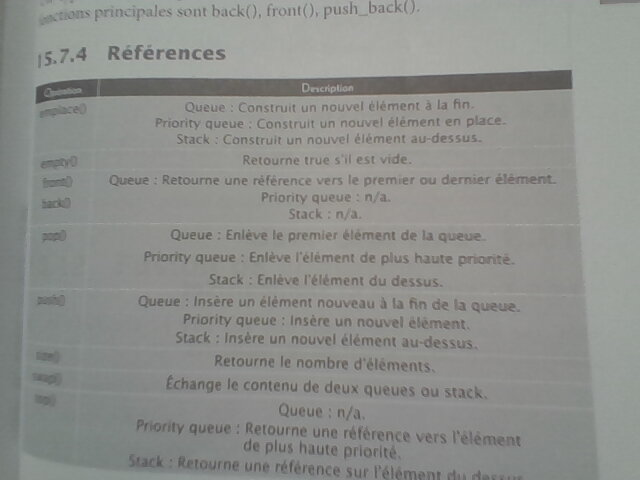
\includegraphics[width=2in]{stack_functions.png}
\end{center}

\section{Tries - Retrieval Trees - AutoComplete}

`std::queue` and `std::stack` containers as part of the standard library, but tries (retrieval trees) are not implemented. 

Here, and example with `std::unordered\_map` or `std::map` for the children nodes,
and custom classes or structs to represent the nodes.

Yet, third-party libraries have implementions of trie data structures.

\begin{verbatim}
#include <unordered_map>

class TrieNode {
public:
    bool isEndOfWord;
    std::unordered_map<char, TrieNode*> children;

    TrieNode() : isEndOfWord(false) {}
};

class Trie {
private:
    TrieNode* root;

public:
    Trie() {
        root = new TrieNode();
    }

    void insert(const std::string& word) {
        TrieNode* curr = root;
        for (char c : word) {
            if (curr->children.find(c) == curr->children.end()) {
                curr->children[c] = new TrieNode();
            }
            curr = curr->children[c];
        }
        curr->isEndOfWord = true;
    }

    bool search(const std::string& word) {
        TrieNode* curr = root;
        for (char c : word) {
            if (curr->children.find(c) == curr->children.end()) {
                return false;
            }
            curr = curr->children[c];
        }
        return curr->isEndOfWord;
    }
};

int main() {
    Trie trie;
    
    // Insert words into the trie
    trie.insert("apple");
    trie.insert("banana");
    trie.insert("cat");
    trie.insert("dog");
    
    // Search for words in the trie
    std::cout << trie.search("apple") << std::endl;  // Output: 1 (true)
    std::cout << trie.search("banana") << std::endl; // Output: 1 (true)
    std::cout << trie.search("cat") << std::endl;    // Output: 1 (true)
    std::cout << trie.search("dog") << std::endl;    // Output: 1 (true)
    std::cout << trie.search("car") << std::endl;    // Output: 0 (false)

    return 0;
}
\end{verbatim}

\subsection{Trie Serialization in JSON or XML}

To save a retrieval tree (trie) and use it later without recreating the tree every time,
you can serialize the tree data structure to a file and then deserialize it when needed.
This allows you to persist the tree structure to disk and load it back into memory when required.

Here are the general steps to achieve this:

1. Serialize the trie: Traverse the trie and convert its nodes and data
into a serialized representation that can be written to a file.
This typically involves converting the tree nodes and their contents into
a suitable format, such as JSON, XML, or a custom binary format.

2. Write the serialized data to a file:
Open a file in write mode and write the serialized data to the file.
You can use file I/O operations provided by the programming language or libraries to accomplish this.

3. Save the file: Close the file and make sure it is saved to a location of your choice,
such as a specific directory.

\textbf{Use the saved trie later}:

1. Read the serialized data from the file:
Open the saved file in read mode and read the serialized data from it.

2. Deserialize the data: Convert the serialized data back into the original trie data structure.
This involves parsing the serialized format and reconstructing the trie nodes and their relationships.

3. Use the trie: Once the trie is deserialized,
you can use it in your program for retrieval or any other operations as needed.

By saving and loading the serialized trie data,
you avoid the need to recreate the entire trie every time your program runs,
improving efficiency and performance.


\section{Trees}

\subsection{Breadth First Search}

\subsection{Depth First Search}


\section{Graphs}

\chapter{Sorting Algorithms}


\section{Bubble Sort}

\section{Quick Sort}


\section{Adjacency Lists}

\subsection{Adjacency Matrix}




\section{Dijsktra Shortest Path}

Below is a C++ implementation of Dijkstra's algorithm for finding the shortest path in a weighted graph.
This implementation uses an adjacency list representation of the graph
and a priority queue (min heap) to efficiently select the next node with the smallest distance.


\begin{verbatim}
#include <iostream>
#include <vector>
#include <queue>
#include <limits>

const int INF = std::numeric_limits<int>::max();

// Node representation in the graph
struct Node {
    int index;
    int distance;

    Node(int idx, int dist) : index(idx), distance(dist) {}

    // Overload the comparison operator for the priority queue
    bool operator>(const Node& other) const {
        return distance > other.distance;
    }
};

// Dijkstra's algorithm for finding the shortest path
std::vector<int> dijkstraShortestPath(const std::vector<std::vector<std::pair<int, int>>>& graph, int source) {
    int n = graph.size();
    std::vector<int> distance(n, INF);
    distance[source] = 0;

    std::priority_queue<Node, std::vector<Node>, std::greater<Node>> pq;
    pq.push(Node(source, 0));

    while (!pq.empty()) {
        Node current = pq.top();
        pq.pop();

        if (current.distance > distance[current.index])
            continue;

        for (const auto& neighbor : graph[current.index]) {
            int newDistance = current.distance + neighbor.second;
            if (newDistance < distance[neighbor.first]) {
                distance[neighbor.first] = newDistance;
                pq.push(Node(neighbor.first, newDistance));
            }
        }
    }

    return distance;
}

int main() {
    int n = 5; // Number of nodes in the graph
    std::vector<std::vector<std::pair<int, int>>> graph(n);

    // Add edges to the graph (format: {destination, weight})
    graph[0].push_back({1, 5});
    graph[0].push_back({2, 3});
    graph[1].push_back({2, 2});
    graph[1].push_back({3, 6});
    graph[2].push_back({3, 7});
    graph[3].push_back({4, 4});

    int source = 0; // Source node

    std::vector<int> shortestDistances = dijkstraShortestPath(graph, source);

    // Print the shortest distances from the source node to all other nodes
    for (int i = 0; i < n; ++i) {
        std::cout << "Shortest dist from node " << source << " to node " << i;
        if (shortestDistances[i] == INF)
            std::cout << "Not reachable" << std::endl;
        else
            std::cout << shortestDistances[i] << std::endl;
    }

    return 0;
}
\end{verbatim}

\section{Algorithms}

\subsection{Accumulate}

\begin{verbatim}
// the algorithm everybody knows. (For_each and accumulate)

#include <numeric>

template<typename T>
T sum_data(const std::vector<T> &d) {
    return std::accumulate(d.begin(), d.end(), T());
}
\end{verbatim}

\subsection{Std::Puts}

Generating a null-terminated string,  a sequence of characters stored in an array
where the end of the string is marked by a null character ('\0'). 
The null character serves as a sentinel value to indicate the end of the string

\begin{verbatim}
#include <format>
#include <string_view>

void print_map(const auto &map, const std::string_view &key_desc = "key",
                                const std::string_view &value_desc = "value")
{
    for (const auto &[key, value] : map) /// structured binding
    {
        std::puts(std::format("{}: '{}' {}: '{}'",
                         key_desc, key, value_desc, value).c_str());

        // this is genious spacing for readability
    }
}

Standard c++20
\end{verbatim}
\subsection{Algorithms and Standard Template Library}

\begin{verbatim}
set<>
vector<>
for_each<>
any_of<>
etc.

A generic set of composable tools

// now, here we are

#include <numeric>
#include <vector>

template<typename Value_Type>
std::vector<Value_Type> get_data(const Value_Type &v1, const Value_type &v2,
                                 const Value_type &v3)
{
    std::vector<Value_Type> data;
    data.push_back(v1);
    data.push_back(v2);
    data.push_back(v3);
    return data;
}

template<typename T>
T sum_data(const std::vector<T> &d) {
    return std::accumulate(d.begin(), d.end(), T());
}

int main() {
    return sum)data(get_data(1,2,3));
}

// But we know the amount of data at compile-time. 
// If only there was some fixed-size container available!

\end{verbatim}

\subsection{Prefer Algorithms Over Loops}

Algorithms communicate meaning and help "const all the things".

Taking a functional approach and using algorithms, we can write cleaner c++.

\begin{verbatim}
// Algorithms end game (before C++20)

const auto has_value
    = std::any_of(begin(container), end(container), 
            greater_than(12));

// Algorithm end game (c++20)

const auto has_value
    = std::any_of(container, greater_than(12));

Next time you are reading through a loop in your codebase,
cross-reference it with the C++ <algorithm> header²
and try to find an algorithm that applies instead.

https://en.cppreference.com/w/cpp/algorithm
\end{verbatim}
